\documentclass{article}
\usepackage[utf8]{inputenc}
\usepackage[english,german]{babel}
\usepackage{utopia}
%\renewcommand{\familydefault}{\sfdefault}
%\fontfamily{phv}\selectfont
\usepackage[margin=1in, a4paper]{geometry}
\usepackage[parfill]{parskip}
\usepackage{makeidx}
\usepackage{hyperref}
\usepackage{graphicx}
\usepackage{fancyhdr}
\usepackage{lastpage}
\usepackage[onehalfspacing]{setspace}

\pagestyle{fancy}
\fancyhf{}
\lhead{Hausaufsatz}
\chead{\today}
\rhead{Patrick Günthard}
\cfoot{\thepage von \pageref{LastPage}}


\title{Hausaufsatz: Geschichte basierend auf einem Zeitungsartikel}
\author{Patrick Günthard}
\date{\today}

\def \nameone {\textit{Jules} } 
\def \nametwo {\textit{Djabel} }

\begin{document}
	
	
	\maketitle
	\section{Artikel}
	
	\textit{Der verwendete Artikel:  \href{http://wat.is/-y0EbCyiC}{In Burundi regiert die Angst vor einem weiteren Bürgerkrieg – Besuch in der Hölle von Bujumbura (watson.ch, 13. 12. 2015)}}
	
	\subsection*{In Burundi regiert die Angst vor einem weiteren Bürgerkrieg – Besuch in der Hölle von Bujumbura}
	
	Das Geräusch von Geschützfeuer gehört in Bujumbura mittlerweile zum Alltag. Das Leben in der sonst so geschäftigen Stadt steht still, auf den Strassen liegen Leichen. Ein Augenzeugenbericht.
	
	\textit{Publiziert: 13.12.15, 13:51 }
	
	Helmenegilde Mwamarariza traut sich kaum noch auf die Strasse. Seit sein 15-jähriger Sohn bei einer Protestaktion gegen die Regierung Burundis getötet wurde, hat er panische Angst, dass auch er zum Schweigen gebracht werden soll.
	
	Während er in seinem Wohnzimmer im Viertel Cibitoke der Hauptstadt Bujumbura seine Geschichte erzählt, sind ganz in der Nähe Schüsse und Explosionen zu hören.
	
	\begin{figure}
	 \centering
	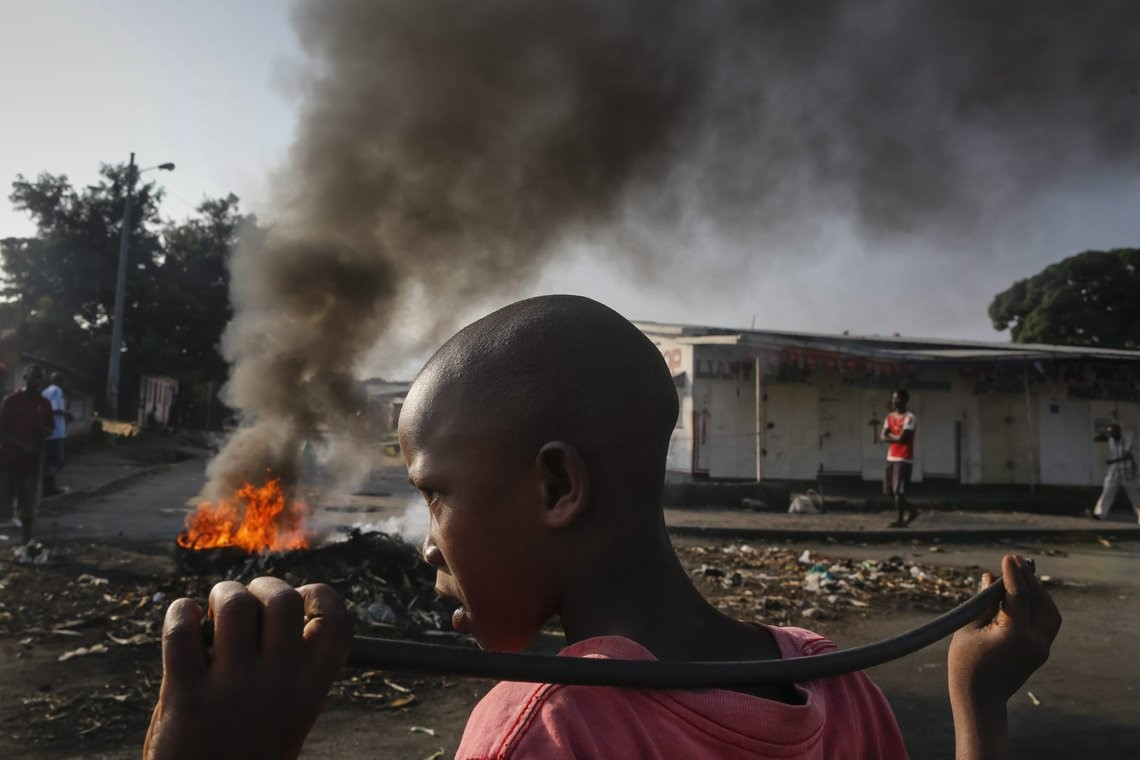
\includegraphics[width=180pt]{img/img1}
	\caption{Ein Junge schaut auf die brennenden Barrikadenreste nach einer Antiregierungs-Demonstration gegen den burundischen Präsidenten Pierre Nkurunziza in Cibitoke im Mai 2015. 
	Bild: DAI KUROKAWA/EPA/KEYSTONE}
	\end{figure}
	
	Die kriegsartigen Geräusche kommen aus dem Nachbarviertel Mutakura, das abgeriegelt worden sein soll, wie sich die Leute in Cibitoke erzählen. «Sie machen Jagd auf die Jugendlichen», heisst es. Aber auch in anderen Teilen Bujumburas sind die von Lehmhäusern mit Wellblechdächern gesäumten Strassen so gut wie leer. 
	
	Kurz nach dem Gespräch mit Mwamarariza werden in der Nähe die von Kugeln durchsiebten Leichen von fünf jungen Männern entdeckt. Sie sollen von Sicherheitskräften getötet worden sein, angeblich, weil sie Attacken geplant hätten. Zwei Tage später, am Freitag, sollen bewaffnete Männer Militärstellungen in mehreren Stadtteilen angegriffen haben, den ganzen Tag über ist Geschützfeuer zu hören.
	
	\textbf{Fotografen müssen mit Festnahme rechnen}
	
	Journalisten haben sich in ihren Hotels verschanzt. Fotografen, die das Grauen dokumentieren und der Welt zeigen wollen, welche unsägliche Gewalt sich gerade in dem kleinen ostafrikanischen Staat mit zehn Millionen Einwohnern abspielt, müssen mit ihrer Festnahme rechnen. Am Ende kommt eine erschreckende Zahl ans Licht: Militärangaben zufolge sollen 87 Menschen ums Leben gekommen sein, darunter auch einige Soldaten und Polizisten.
	
	
	\begin{figure}
		  \centering
		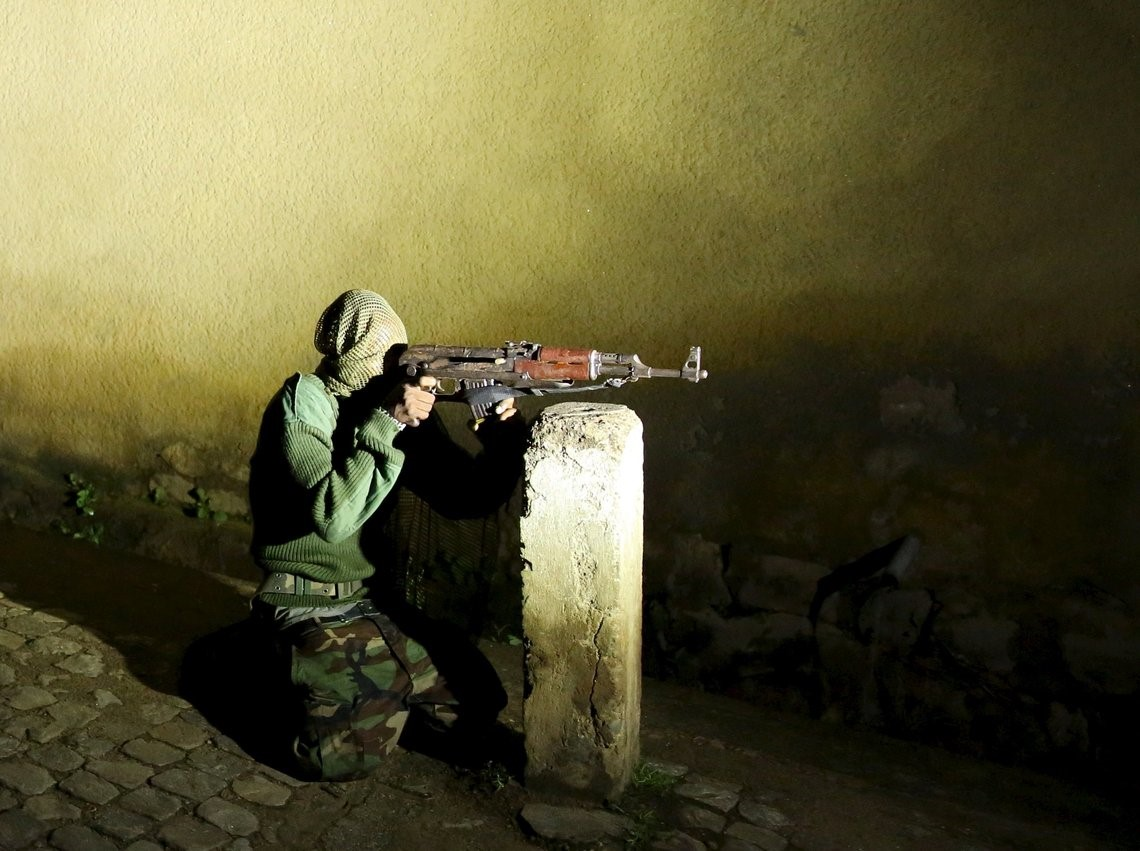
\includegraphics[width=180pt]{img/img2}
		\caption{Ein bewaffneter der Bürgerwehr im Zentrum von Bujumbura im November 2015. Bild: GORAN TOMASEVIC/REUTERS}
	\end{figure}
	
	Die Gesellschaft für bedrohte Völker (GfbV) forderte am Sonntag die Einsetzung einer unabhängigen Untersuchungskommission des UNO-Hochkommissariats für Menschenrechte, um die Todesfälle aufzuklären. Augenzeugenberichte deuteten darauf hin, dass junge Menschen willkürlich hingerichtet worden seien. Sie seien von Sicherheitskräften auf die Strasse getrieben und zum Teil noch mit gefesselten Händen erschossen worden.
	
	Erst vor einem Jahrzehnt ging in Burundi ein entsetzlicher Bürgerkrieg mit 300'000 Toten zu Ende. Lange sollte der Frieden nicht währen. Für die Menschen in der ehemaligen belgischen Kolonie ist heute der Horror real, Tag für Tag.
	
	Der UNO-Sicherheitsrat reagierte ebenfalls und teilte mit, die Mitglieder seien «zutiefst besorgt» über die Entwicklungen. Die Schuldigen müssten endlich zur Verantwortung gezogen werden – notfalls müssten weitere Schritte eingeleitet werden. Aber wer sind die Schuldigen?
	
	\textbf{Ein Rückblick: Immer wieder Blutbäder}
	
	Im April kündigt Präsident Pierre Nkurunziza an, bei der anstehenden Wahl für eine dritte Amtszeit kandidieren zu wollen, obwohl dies in der Verfassung nicht vorgesehen ist. Viele Menschen reagieren wütend, es kommt zu ersten gewaltsamen Zusammenstössen mit der Polizei. Nkurunziza gibt sich unbeeindruckt vom Blut in den Strassen. Im Juli wird er im Amt bestätigt - die Opposition boykottierte die Wahl.
	
	
	\begin{figure}
		  \centering
		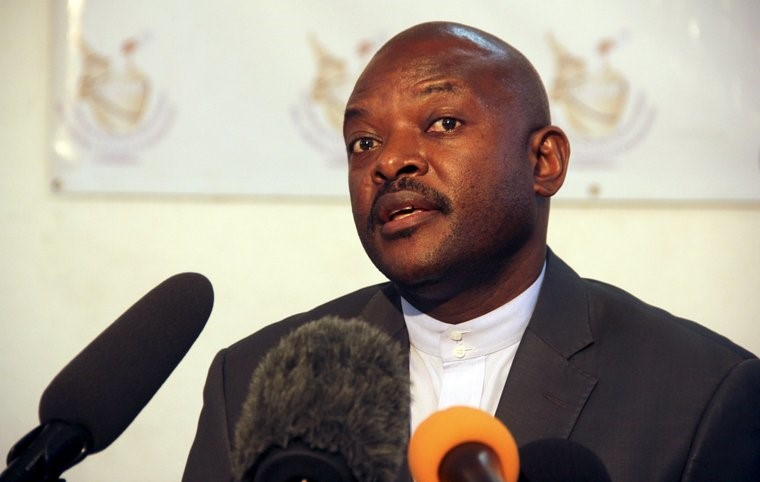
\includegraphics[width=180pt]{img/img3}
		\caption{Ein von den blutigen Protesten unberührter Präsident: Pierre Nkurunziza. Bild: JEAN PIERRE HARERIMANA/REUTERS}
	\end{figure}
	
	Viele wollen Nkurunzizas Gebaren nicht hinnehmen, es bilden sich bewaffnete Gruppen, die versuchen, den Präsidenten zu stürzen. Immer wieder kommt es zu Blutbädern. Die Polizei reagiert ohne Erbarmen, sie schiesst und lässt sogar manchmal Leichen verschwinden.
	
	«Unser einziger Trost ist, dass wir ihn begraben konnten», sagt eine Angehörige von Remy Nkengurutse. Demnach wurde der 29-jährige Aktivist in der vergangenen Woche von der Polizei niedergeschossen, als er gerade aus einem Bus stieg. «Andere Leute verschwinden einfach spurlos.»
	
	\begin{figure}
		  \centering
		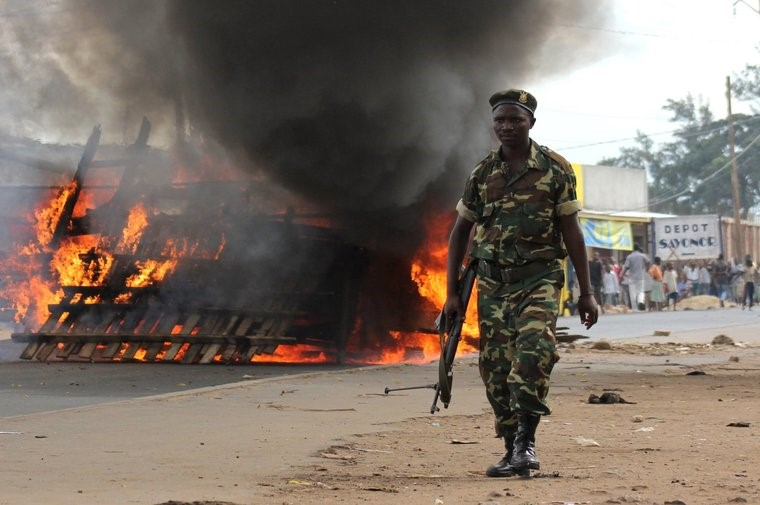
\includegraphics[width=180pt]{img/img4}
		\caption{Ein Soldat läuft an brennenden Barrikaden vorbei: Der Protest gegen Nkurunzizas dritte Amtszeit wurde blutig niedergeschlagen. Bild: JEAN PIERRE HARERIMANA/REUTERS}
	\end{figure}
	
	Mittlerweile bekommen viele Bürger in Cibitoke und Mutakura schon Angst, wenn jemand nur das Wort «Polizei» ausspricht. Die beiden Arbeiterviertel gelten als Hochburgen der Opposition, sind voll von aufgebrachten Jugendlichen. Zusammenstösse mit der Polizei – und deren mutmasslichen Verbündeten, der Jugendorganisation «Imbonerakure» der Regierungspartei CNDD-FDD – gehören zum Alltag.
	
	Die Vorwürfe gegen die Polizei reichen von Plünderungen bis hin zu Vergewaltigungen. «Ich werde der Polizei nie wieder vertrauen», sagt eine 15-Jährige, die nach eigenen Worten von einem Beamten in ihrem Haus vergewaltigt wurde.
	
	Gewalt auf beiden Seiten
	Doch Gewalt gibt es auf beiden Seiten. Auch Polizisten und Imbonerakure-Mitglieder werden ständig bedroht, eine 24-jährige Kollegin sei erst kürzlich vergewaltigt, brutal verstümmelt und ermordet worden, sagt Imbonerakure-Chef Dennis Karera.
	
	Der trauernde Vater Helmenegilde Mwamarariza wischt sich derweil die Tränen aus den Augen. Auf einem Beistelltisch steht das Foto seines Sohnes Jean Nepo. Da lacht er, schaut fröhlich aus.
	
	\begin{figure}
		  \centering
		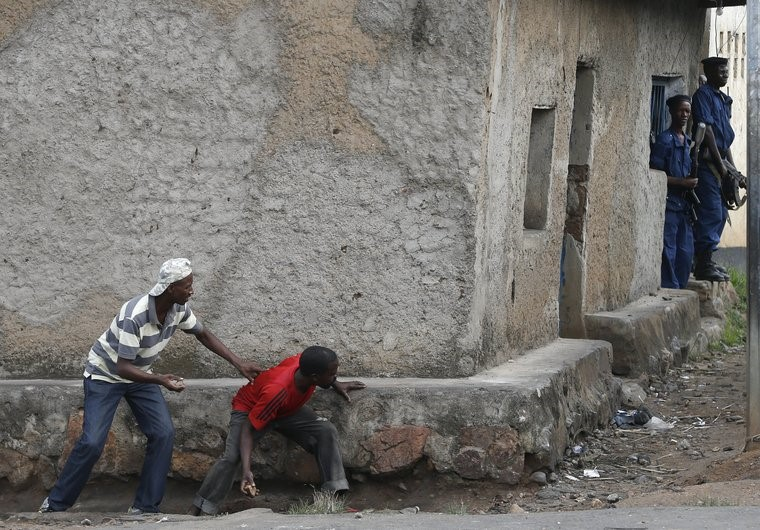
\includegraphics[width=180pt]{img/img5}
		\caption{Die Gewalt kommt von beiden Seiten. Bild: GORAN TOMASEVIC/REUTERS}
	\end{figure}
	
	Am 26. April 2015 wurde der Jugendliche von einem Polizisten mit einer Waffe bedroht. Jean Nepo sei in die Knie gegangen, habe um sein Leben gefleht, erzählten Augenzeugen später. Aber der Polizist habe einfach abgedrückt. Der Schüler war das erste Opfer der neuen Gewaltwelle. Mittlerweile sind ihm Hunderte in den Tod gefolgt. 
	
	\textit{(sda/dpa)}
	
	\clearpage
	
	\section{Text}
	\subsection*{Die Angst vor dem Krieg}
		Diesen Morgen ging \nameone eine Strasse hinab. Dieser Stadtteil von Bujumbura, der Hauptstadt Burundis war sonst immer sehr ruhig. In der letzten Zeit hat sich jedoch viel geändert. Bewaffnete Männer prägen das Strassenbild und raus geht nur, wer auch muss.
		
		Der Polizei und dem Militär kann man nicht mehr trauen. \nameone hörte täglich  von willkürlichen Exekutionen und Vergewaltigungen. Darum dachte er, es wäre schlauer, diesen Leuten aus dem Weg zugeht.
		
		Als er ein Lastwagen der Armee in die Strasse einbiegen ssah welcher er entlang lief, verlangsamte er seinen Gang, blieb stehen und fing dann an in eine Seitenstrasse zu rennen. Gerade noch rechtzeitig kam er davon und schaffte es zurück zu seiner Barackensiedlung wo er wohnte. 
		
		Das Leben in Burundi ist hart. Fast die Hälfte der Leute können weder lesen noch Schreiben. \nameone hatte das Glück, einige Jahre zur Schule gehen zu dürfen, jedoch nur bis er gerade genug alt war um arbeiten zu können. Viele seiner Freunde mussten schon als Kind arbeiten, manchmal waren sie kaum 10 Jahre alt.
		
		Er ging zum Haus von \nametwo, einen seiner besten Freunde. \nametwo traute sich kaum noch aus dem Haus seit dem im April dieses Jahres ein Junge auf offener Strasse von der Polizei hingerichtet wurde. Er meinte, er wolle nicht raus, als \nameone ihn fragte wann er zuletzt Tageslicht gesehen hatte.
		
		In der Ferne hörte man Gewehrfeuer und Explosionen. \nametwo zuckte jedes Mal zusammen. Er ist einige Jahre älter als \nameone und daher hat den Bürgerkrieg welcher vor erst 10 Jahre geendet hatte noch bewusster miterlebt. Die Angst, dass der Krieg von neuem beginnt ist allgegenwärtig. 
	
		Neben der Angst war auch Wut da. Wut gegen den Präsidenten, Wut gegen das korrupte System. Die willkürliche Gewalt war allgegenwärtig und \textit{Pierre Nkurunziza}, der Präsident interessierte sich überhaupt nicht dafür. Es gab sogar Gerüchte, er würde die Vergewaltigungen und Erschiessungen selbst befehlen. An diesem Nachmittag hatte die Opposition eine Demonstration in der Innenstadt angekündigt. \nameone beschloss, dorthin zu gehen. Der Versuch \nametwo dazu zu überreden ebenfalls zu gehen scheiterte.
		
		Als \nameone am Ort der Demonstration ankam, wütete bereits eine heftige Strassenschlacht. Es wurden bereits Barrikaden errichtet und alle paar Minuten gab es Schiessereien. 
		
		Irgendwann wurde es plötzlich ruhig. Und dann hörte \nameone einen Knall. Und dann noch einen. Er schaute um die Ecke und sah die Soldaten langsam auf sich zukommen. Um die Soldaten lagen mehrere Leichen von Jugendlichen, meist keine 16 Jahre alt, erschossen oder erschlagen.
		
		Er versteckte sich hinter einem ausgebrannten Auto und wartete, bis die Soldaten verschwunden waren. Als sie weg waren, lief er langsam auf die immer noch brennenden Barrikaden zu. \nameone schaute auf den Boden und erschrak. Er hatte das Gefühl, er würde jemanden den er kennt unter den Leichen erkennen. Er trat näher und sah das Gesicht von \nametwo. 
		
		
		
	
\end{document}